\documentclass[11pt]{article}  
\usepackage[left=3cm, right=3cm, bottom=3cm]{geometry}           	
\usepackage[parfill]{parskip}    		
\usepackage{graphicx}
\usepackage{cleveref}
\usepackage[export]{adjustbox}
\usepackage{mathabx}
\usepackage{subfig}	
\usepackage{url}						
\renewcommand{\baselinestretch}{1}
\usepackage[font=footnotesize,labelfont=bf]{caption}
\usepackage{float}
\usepackage[font=scriptsize]{caption}

\title{CS5014 - Machine Learning 
\\ \vspace{5mm} \Large P2 - Classification of object colour 
\\ using optical spectroscopy 
\\~\\ Report}
\author{140014952}

\small %\date{}
 
\begin{document}
	\maketitle

	\section{Overview}
		The objectives of this practical were to come up with classification model for binary and multi-class classification problems. This submission investigates both binary and multi-class tasks. The solution python scripts can be found in \textit{/binaryML/} and \textit{/multiclassML/} directories. 

		As later sections suggest, the amount of features it takes to determine the class for each task is very low. This is hypothesized based on input analysis and later machine learning observations support these hypotheses. 

	\section{Cleaning Data and Feature Extraction}
		As the very first step input data were split into training and testing data. The analysis were first done on the training sets. 
	\section{Data Analysis and Visualization}

		To visualize training data X it was plotted with provided wavelength data that contains information about each feature wave length. Additionally, Y training set was used to indicate visually how colours are distributed and can be distinguished. This gave insights as to which features are likely to be good indicators for predicting the colour. Plots for both binary and multi-class data were generated. 

		\subsection{Binary Classification}
			Fig.\ref{fig:binary} shows that there is a clear distinction between red and green colours in terms of features. From the same figure it can be said feature values between 400 and 500 wavelength are more or less shared between both red and green colours. Around 600 wavelength both colour features overlap. Similarly, towards the final features similar observations can be made. The graph insights suggest that overlapping features are not great for determining the class because a feature value can be shared by both colours therefore reducing possibility of determining the right colour. However, a single feature that is around 520 or 640 should be good enough to determine the class. From fig.\ref{fig:binary} it is clear that those wavelength values are distinct to each colour.

			\begin{figure}[H]
				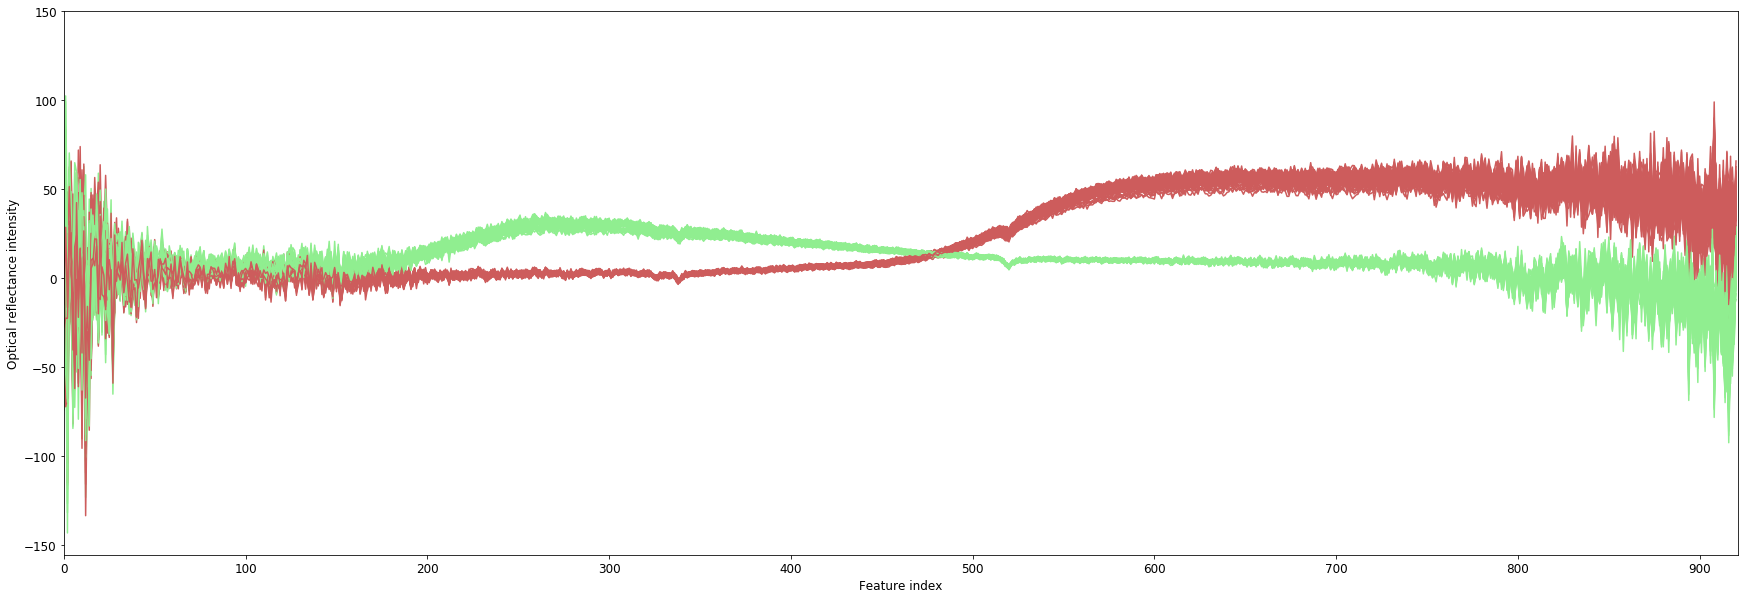
\includegraphics[width=1\textwidth]{png/binary_default}
				\caption{Input feature visualization for binary classification task. Red and green predicting features are indicated by colour.}
				\label{fig:binary}
			\end{figure}

		\subsection{Multi-Class Classification}

		\begin{figure}[H]
			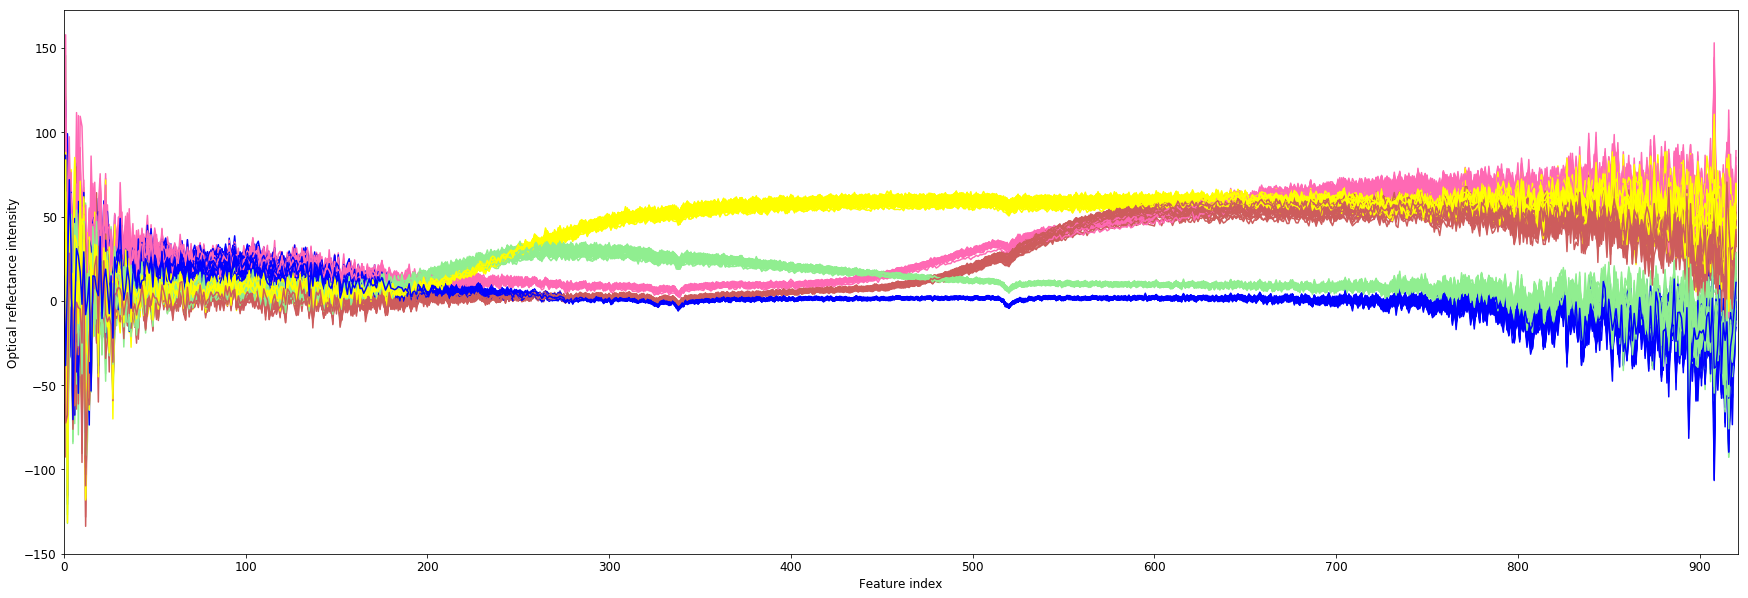
\includegraphics[width=1\textwidth]{png/multi_default}
			\caption{}
			\label{fig:milti}
		\end{figure}

	\section{Preparing Inputs and Choosing Features}
	\section{Selecting and Training Classification Models}
	\section{Evaluating and Comparing Model Performance}
	\section{Result Discussion}


	\section{Conclusion}
	
\end{document}  